% This work is licensed under the Creative Commons Attribution-NonCommercial 4.0 International License.
% To view a copy of this license, visit http://creativecommons.org/licenses/by-nc/4.0/
% or send a letter to Creative Commons, PO Box 1866, Mountain View, CA 94042, USA.

% !TEX TS-program = xelatex

\documentclass[../Main/chem532-notes.tex]{subfiles}
\begin{document}

\chapter{The full CI equations and Slater rules}

\section{The FCI equations and their solution}

In this section we will derive the equations that determine the coefficients in the FCI wave function.
For convenience, we will introduce a short-hand notation for a Slater determinant $\Phi_{ijk\cdots}(x_1,x_2,\ldots,x_N)$ where we condense all the orbital indices ${ijk\cdots}$ to a multi-index $I = \{i_1,i_2,i_3,\cdots\}$ with $i_1 < i_2 < i_3 < \ldots$, so that we can write determinants with only one label as $\Phi_I$.\mnote{The index $I$ is also called a \textit{string} of indices $I = \{ i_1,i_2, \ldots, i_N \}$ that indicate the occupied spin orbitals.}
Then the FCI wave function can be written as
\begin{equation}
\ket{\Psi_{\mathrm{FCI}}} = \sum_I c_I \ket{\Phi_I}.
\end{equation}

To derive the FCI equations we first have to establish the properties of the basis of Slater determinant. Recall that a determinant may be written as
\begin{equation}
\begin{split}
\Phi_{i_1 i_2 \cdots i_N}(x_1,x_2,\ldots,x_N) &= \frac{1}{\sqrt{N!}}
\begin{vmatrix}
\psi_{i_1}(x_1) & \psi_{i_1}(x_2) & \cdots & \psi_{i_1}(x_N) \\
\psi_{i_2}(x_1) & \psi_{i_2}(x_2) & \cdots & \psi_{i_2}(x_N) \\
\vdots & \vdots & \ddots &  \vdots \\
\psi_{i_N}(x_1) & \psi_{i_N}(x_2) & \cdots & \psi_{i_N}(x_N) \\
\end{vmatrix} \\
&= \frac{1}{\sqrt{N!}}
\sum_{\pi}^{N!} (-1)^{p_\pi} P_{\pi}\left[
\psi_{i_1}(x_1) \psi_{i_2}(x_2) \cdots \psi_{i_N}(x_N)
\right],
\end{split}
\end{equation}
where $\pi$ labels a permutation, $(-1)^{p_\pi}$ is the parity of the permutation $\pi$, and $P_{\pi}$ is a permutation operator that acts on the electron coordinates.\mnote{For example, for two indices $\pi = [(1,2), (2,1)]$ and $p_\pi = [0,1]$.}

The overlap integral $\braket{\Phi_I|\Phi_I}$ for a generic determinant $\Phi_I$ may be written as
\begin{equation}
\begin{split}
\braket{\Phi_I|\Phi_I} &= \frac{1}{N!}
\sum_{\pi}^{N!} \sum_{\pi'}^{N!} (-1)^{p_\pi + p_{\pi'}} \int dx_1 dx_2 \cdots dx_N \\
&
P_{\pi}\left[
\psi_{i_1}^{*}(x_1) \cdots \psi_{i_N}^{*}(x_N)
\right]
P_{\pi}\left[
\psi_{i_1}(x_1) \cdots \psi_{i_N}(x_N)
\right].
\end{split}
\end{equation}
Since the spin-orbital basis is assumed to be orthonormal,\mnote{$\braket{\psi_i|\psi_j} = \delta_{ij}$.} the integrals for each separate variable must contain the square of the same spin orbital to get a non-zero result.
This happens when the two permutations coincide, $\pi = \pi'$, in which case the integral simplifies to:
\begin{equation}
 \int dx_1 dx_2 \cdots dx_N 
P_{\pi}\left[
|\psi_{i_1}(x_1)|^2 |\psi_{i_2}(x_2)|^2 \cdots |\psi_{i_N}(x_N)|^2
\right] = 1.
\end{equation}
Summing over all permutations we have
\begin{equation}
\braket{\Phi_I | \Phi_I} = \frac{1}{N!}
\sum_{\pi}^{N!} 1 =  \frac{N!}{N!} = 1.
\end{equation}

\begin{problem}[Orthogonality of Slater determinants]
Show that two determinants $\Phi_I$ and $\Phi_J$ that differ by one or more spin orbital have zero overlap
\begin{equation}
\braket{\Phi_I | \Phi_J} = 0.
\end{equation}
\end{problem}
The orthonormality condition for the Slater determinants may be summarized as:
\begin{equation}
\braket{\Phi_I | \Phi_J} = \delta_{IJ}.
\end{equation}

We can now proceed to derive the FCI equations.
Plugging in the FCI wave function in the Schr\"{o}dinger equation we obtain
\begin{equation}
\hat{H} \sum_I c_I \ket{\Phi_I} = E \sum_I c_I \ket{\Phi_I}.
\end{equation}
Projecting onto the left with $\bra{\Phi_J}$ and rearranging terms we get
\begin{equation}
 \sum_I \braket{\Phi_J |\hat{H} | \Phi_I} c_I = E \sum_I \underbrace{\braket{\Phi_J | \Phi_I}}_{\delta_{IJ}} c_I,
\end{equation}
which may be simplified to 
\begin{equation}
 \sum_I H_{IJ} c_I = E c_J,
\end{equation}
with the matrix elements $H_{IJ}$ defined as $H_{IJ} = \braket{\Phi_J |\hat{H} | \Phi_I}$.
This is an eigenvalue problem that can be written compactly as
\begin{equation}
\mathbf{H}\mathbf{C} = \mathbf{C} \mathbf{E},
\end{equation}
where $\mathbf{H}$ is a matrix of dimension $N_{\mathrm{FCI}} \times N_{\mathrm{FCI}}$, where $N_{\mathrm{FCI}}$ is the number of FCI determinants.
To solve this equation we have to derive equations for the matrix elements of the Hamiltonian operator $H_{IJ} = \braket{\Phi_J |\hat{H} | \Phi_I}$. The set of rules that determine the value of these matrix elements are called \textbf{Slater rules}.

\section{Deriving the FCI equations using the Lagrangian approach}
In this section we will derive the FCI equations using a different approach based on the formalism of Lagrange multipliers.
In this approach we seek to minimize the Rayleigh--Ritz functional
\begin{equation}
E_\mathbf{RR}[\Psi] = \frac{\bra{\Psi} \hat{H} \ket{\Psi}}{\braket{\Psi|\Psi}}.
\end{equation}
Note that the denominator $\braket{\Psi|\Psi}$ is necessary to guarantee that the functional is valid irrespective of the way we normalize the wave function $\Psi$.
If the smallest eigenvalue of the Hamiltonian ($E_0$) is bound, that is, $E_0 > - \infty$, then minimization of $E_\mathrm{RR}[\Psi]$ with respect to $\Psi$ will give the lowest eigenvalue and eigenstate ($\Psi_0$) of the Hamiltonian 
\begin{equation}
\min_{\Psi} E_\mathbf{RR}[\Psi] = E_0.
\end{equation}
The minimum of $E_\mathrm{RR}[\Psi]$ is obtained by solving the set of equations
\begin{equation}
\frac{\partial E_\mathrm{RR}[\Psi]}{\partial c_I} = 0.
\end{equation}
This approach is a bit clumsy because the expression that we want to minimize contains the quantity $\braket{\Psi|\Psi}$ in the denominator.

The Lagrangian approach offers a more direct way to find the FCI equations.
To begin with, we write a Lagrangian, that is a function that contains the quantity that we want to minimize and the constraints that we need to satisfy.

\begin{example}[Minimization of a function of two variables with a constraint]
Let us consider the problem of minimizing the function $f(x,y) = x^2 + 2 y^2$ with the constraint that $x + y = 2$.
We rewrite the constraint as a function $g(x,y) = x + y - 2$ and we will try to impose $g(x,y) = 0$.
Consider the Lagrangian function of three independent variables $(x,y,\lambda)$:
\begin{equation}
\mathcal{L}(x,y,\lambda) = f(x,y) - \lambda g(x,y) =  x^2 + 2 y^2 - \lambda (x + y - 2).
\end{equation}
The stationary point of $\mathcal{L}(x,y,\lambda)$ with respect to the variables $x$, $y$, and $\lambda$ corresponds to:
\begin{align}
\frac{\partial \mathcal{L}(x,y,\lambda)}{\partial x} &= 2 x - \lambda = 0 \label{eq:hf:lagrange1}\\
\frac{\partial \mathcal{L}(x,y,\lambda)}{\partial y} &= 4 y - \lambda = 0 \label{eq:hf:lagrange2}\\
\frac{\partial \mathcal{L}(x,y,\lambda)}{\partial \lambda} &= g(x,y)  = 0.\label{eq:hf:lagrange3}
\end{align}
From Eqs.~\eqref{eq:hf:lagrange1} and \eqref{eq:hf:lagrange2} we obtain:
\begin{equation}
x = 2y,
\end{equation}
which combined with Eq.~\eqref{eq:hf:lagrange3} gives: 
\begin{equation}
g(2y,y)  = 2y + y - 2 = 0 \quad \Rightarrow \quad y = \frac{2}{3},
\end{equation}
and $x = \frac{4}{3}$.
\end{example}

The FCI Lagrangian is given by the energy minus the normalization constraint
\begin{equation}
\begin{split}
\mathcal{L}[\Psi] & = \underbrace{\bra{\Psi} \hat{H} \ket{\Psi}}_{\text{energy}} - \underbrace{\lambda (\braket{\Psi|\Psi} - 1)}_{\text{normalization constraint}} \\
& = \sum_{IJ} c_I^{*} H_{IJ} c_J - \lambda (\sum_{I} |c_I^2| - 1).
\end{split}
\end{equation}
Taking the derivative of $\mathcal{L}[\Psi]$ with respect to $c_I^{*}$ gives
\begin{equation}
\frac{\partial \mathcal{L}[\Psi] }{\partial c_I^{*}} = \sum_{J} H_{IJ} c_J - \lambda c_I,
\end{equation}
from which we conclude that the FCI vector $\mathbf{c}$ must satisfy the eigenvalue equation
\begin{equation}
\sum_{J} H_{IJ} c_J = \lambda c_I.
\end{equation}




\section{Slater rules}
In this section we look at how can we compute matrix elements of the Hamiltonian $\bra{\Phi_I} \hat{H} \ket{\Phi_J}$, where $\Phi_I$ and $\Phi_J$ are two determinants built out of the same orthonormal spin orbital basis. \mnote{More general rules exist for nonorthonormal spin orbitals, and when $\Phi_I$ and $\Phi_J$ use different set of spin orbitals.}
For convenience we will write the electronic Hamiltonians as
\begin{equation}
\hat{H} = V_\mathrm{NN} + \hat{H}_1 + \hat{H}_2,
\end{equation}
where
\begin{align}
V_{NN} &= \sum_{A}^{M} \sum_{B > A}^{M} \frac{Z_A Z_B}{r_{AB}}\\
\hat{H}_1 &= -\frac{1}{2} \sum_i^N \nabla^2_i
- \sum_{i}^{N} \sum_{A}^{M} \frac{Z_A}{r_{iA}} = \sum_i \hat{h}(i)\\
\hat{H}_2 &= \sum_{i}^{N}\sum_{j > i}^{N} \frac{1}{r_{ij}} = \sum_{i}^{N}\sum_{j > i}^{N} \hat{v}(i,j).
\end{align}

\subsection{Matrix elements of the scalar term}
The simplest matrix element is that of the scalar term ($V_{NN}$), which can be derived using only the orthonormality condition of the Slater determinant basis
\begin{equation}
\bra{\Phi_I} V_\mathrm{NN} \ket{\Phi_J}
= V_\mathrm{NN} \braket{\Phi_I | \Phi_J} = V_\mathrm{NN} \delta_{IJ}.
\end{equation}

\subsection{Matrix elements of the Hamiltonian}
Let us consider the matrix element of the one-body operator:
\begin{equation}
\begin{split}
\bra{\Phi_I} \hat{H}_1 \ket{\Phi_I} &= \frac{1}{N!}
\sum_{\pi \pi'}^{N!} \sum_j (-1)^{p_\pi + p_{\pi'}} \int dx_1 dx_2 \cdots dx_N \\
&
P_{\pi}\left[
\psi_{i_1}^{*}(x_1) \cdots \psi_{i_N}^{*}(x_N)
\right]
\hat{h}(x_j)
P_{\pi'}\left[
\psi_{i_1}(x_1) \cdots \psi_{i_N}(x_N)
\right].
\end{split}
\end{equation}
In this case the only permutations that give nonzero contributions are those for which $\pi = \pi'$.
Otherwise, there would be one or more mismatched spin orbitals. For example, consider the case of a permutation $\pi'$ that swaps coordinates $x_1 \leftrightarrow x_2$ while $\pi$ is the identity. The term with the operator $\hat{h}(x_1)$
\begin{equation}
\begin{split}
\int dx_1 dx_2 \cdots \,
\psi_{i_1}^{*}(x_2) \psi_{i_2}^{*}(x_1) \cdots
\hat{h}(x_1)
\psi_{i_1}(x_1) \psi_{i_2}(x_2)\cdots  \\
= \int dx_1 \, \psi_{i_2}^{*}(x_1) \hat{h}(x_1) \psi_{i_1}(x_1)
\times \underbrace{\int dx_2 \, \psi_{i_1}^{*}(x_2) \psi_{i_2}(x_2)}_{= 0} \times \cdots = 0.
\end{split}
\end{equation}
We also get zero if the permutation mixes two variables not involved with the operator $\hat{h}$ as in the case of the permutation $\pi' \equiv (x_2 \leftrightarrow x_3)$ 

\begin{equation}
\begin{split}
\int dx_1 dx_2 \cdots \,
\psi_{i_1}^{*}(x_1) \psi_{i_3}^{*}(x_2) \cdots
\hat{h}(x_1)
\psi_{i_1}(x_1) \psi_{i_2}(x_2) \cdots  \\
= \int dx_1 \, \psi_{i_1}^{*}(x_1) \hat{h}(x_1) \psi_{i_1}(x_1)
\times \underbrace{\int dx_2 \, \psi_{i_3}^{*}(x_2) \psi_{i_2}(x_2)}_{= 0} \times \cdots = 0.
\end{split}
\end{equation}
Since for any permutation $P_{\pi} \sum_j\hat{h}(x_j) = \sum_j\hat{h}(x_j)$, we may combine the permutation operators into a single term
%Since the Slater determinant contains a sum over all permutations of indices, we can consider only the effect of the one-electron operator acting of the wave functions labeled by the coordinate $x_1$.
%This means we can replace  $\sum_j \hat{h}(j)$ with $N \hat{h}(1)$.
\begin{equation}
\begin{split}
\bra{\Phi_I} \hat{H}_1 \ket{\Phi_I} &= \frac{1}{N!}
\sum_{\pi}^{N!} \int dx_1 dx_2 \cdots dx_N \\
&
P_{\pi}\left\{
\psi_{i_1}^{*}(x_1) \cdots \psi_{i_N}^{*}(x_N)
\left[\sum_j\hat{h}(x_j)\right]
\psi_{i_1}(x_1) \cdots \psi_{i_N}(x_N)
\right\}.
\end{split}
\end{equation}
Each permutation of the integral will give a contribution equal to:
\begin{equation}
\sum_j^{N} \int dx \, \psi_{i_j}^{*}(x) \hat{h}(x) \psi_{i_j}(x) 
= \sum_j^{N} \bra{\psi_{i_j}} \hat{h} \ket{\psi_{i_j}} = \sum_i^{\rm occ} \bra{\psi_i}\hat{h}\ket{\psi_i},
\end{equation}
and since there are $N!$ permutations, we find that 
\begin{equation}
\bra{\Phi_I} \hat{H}_1 \ket{\Phi_I} = \frac{1}{N!}
\sum_{\pi}^{N!}   \sum_i^{\rm occ} \bra{\psi_i}\hat{h}\ket{\psi_i} =  \sum_i^{\rm occ} \bra{i}\hat{h}\ket{i}.
\end{equation}
In the last term we introduced the abbreviated notation $\bra{i}\hat{h}\ket{i} \equiv \bra{\psi_i}\hat{h}\ket{\psi_i}$.
The derivation of the two-electron contribution is more involved, and it gives the following result:
\begin{equation}
\bra{\Phi_I} \hat{H}_2 \ket{\Phi_I} = \sum_{i} \sum_{j < i}
\left[ \braket{i j|i j} -  \braket{i j|j i}\right],
\end{equation}
where the quantity $\braket{i j|k l}$ is a two-electron integral in \textbf{physicist notation}:
\begin{equation}
\braket{i j | k l} = \int dx_1 dx_2 \psi_{i}^{*}(x_1) \psi_{j}^{*}(x_2) \hat{v}(x_1,x_2) \psi_{k}(x_1) \psi_{l}(x_2).
\end{equation}
If we introduce the antisymmetrized two-electron integral:
\begin{equation}
\aphystei{i j}{k l}  = \braket{i j|k l} - \braket{i j|l k},
\end{equation}
then it is possible to rewrite as an unconstrained double sum
\begin{equation}
\bra{\Phi_I} \hat{H}_2 \ket{\Phi_I} = \sum_{i} \sum_{j < i}
\aphystei{i j}{i j} = \frac{1}{2} \sum_{ij} \aphystei{i j}{i j},
\end{equation}
since the term that corresponds to $i = j$ is null\mnote{This is simple to see: $\braket{i i\| i i} = \braket{i i| i i} - \braket{i i| i i} = 0$.} and $\aphystei{j i}{j i} = \aphystei{i j}{i j}$.
%The permutation operators in the integral may divided into two types.
%Permutations that shuffle the indices $x_2,x_3,\ldots,x_N$ or those that exchange $x_1$ and shuffle  
%\\
%&= \frac{(N-1)!}{(N-1)!}
%\sum_j \int dx_1 \psi_{j}^{*}(x_1) \hat{h}(x_1) \psi_{j}(x_1) 
%= \sum_j \braket{j | \hat{h} | j} = \sum_{j} h_{jj}.

In summary we can express the diagonal element of the Hamiltonian matrix as
\begin{iequation}
\label{eq:slater_rule1}
\bra{\Phi_I} \hat{H}_1 \ket{\Phi_I} = V_\mathrm{NN}
+ \sum_i^{\rm occ} \bra{i}\hat{h}\ket{i}
+ \frac{1}{2} \sum_{ij}^{\rm occ} \aphystei{i j}{i j},
\end{iequation}
where each sum is over the set of occupied molecular orbitals in $\Phi_I$ [denotes as $\mathrm{occ}(\Phi_I)$]. 

\begin{example}[Energy of a single electron]
Consider the determinant for a single electron:
\begin{equation}
\ket{\psi_1}.
\end{equation}
The energy is then given by:
\begin{equation}
\bra{\psi_1} \hat{H} \ket{\psi_1} = \bra{1} \hat{h} \ket{1} + \frac{1}{2} \underbrace{\aphystei{11}{11}}_{=0} = \bra{1}\hat{h}\ket{1}.
\end{equation}
\end{example}

\begin{example}[Energy of a pair of electrons in a closed-shell configuration]
Let us consider the determinant:
\begin{equation}
\ket{\Phi_I} = \ket{\psi_1 \psi_{\bar{1}}}
\end{equation}
The energy is given by:
\begin{equation}
\begin{split}
\bra{\Psi_I} \hat{H} \ket{\Psi_I} =& \bra{\psi_1}\hat{h}\ket{\psi_1} + \bra{\psi_{\bar{1}}} \hat{h} \ket{\psi_{\bar{1}}}\\ 
&+ \frac{1}{2} \left[ 
\aphystei{\psi_1 \psi_1}{\psi_1 \psi_1}
+ \aphystei{\psi_1\psi_{\bar{1}}}{\psi_1\psi_{\bar{1}}} 
+ \aphystei{\psi_{\bar{1}}\psi_1}{\psi_{\bar{1}}\psi_1} + \aphystei{\psi_{\bar{1}}\psi_{\bar{1}}}{ \psi_{\bar{1}}\psi_{\bar{1}}}\right] \\
=& 2 \bra{\phi_1}\hat{h}\ket{\phi_1} + \braket{\phi_1 \phi_1| \phi_1 \phi_1},
\end{split}
\end{equation}
where we have eliminated two-electron integrals that are zero due to a mismatch in the spin function.
\end{example}

To simplify this notation, sometimes we will use the \textbf{Coulomb integral} ($J_{ij}$)
\begin{equation}
J_{ij} =\braket{ij|ij} = 
\int dx_1 dx_2 \frac{|\psi_{i}(x_1)|^2 |\psi_{j}(x_2)|^2 }{|\mathbf{r}_1 - \mathbf{r}_2|}
= \int dx_1 dx_2 \frac{|\phi_{i}(\mathbf{r}_1)|^2 |\phi_{j}(\mathbf{r}_2)|^2 }{|\mathbf{r}_1 - \mathbf{r}_2|},
\end{equation}

%\braket{\phi_i \phi_j}{\phi_i \phi_j} = 
%\int d\mathbf{r}_1 d\mathbf{r}_2 \frac{|\phi_{i}(x_1)|^2 |\phi_{j}(x_2)|^2 }{|\mathbf{r}_1 - \mathbf{r}_2|}
which is just Coulomb's law for a two charges with density distribution $\rho_i(\mathbf{r}) = |\phi_{i}(\mathbf{r})|^2$ and $\rho_j(\mathbf{r}) = |\phi_{j}(\mathbf{r})|^2$.
We can also define the \textbf{exchange} integral ($K_{ij}$) as
\begin{equation}
K_{ij} =\braket{ij|ji} = 
\int dx_1 dx_2 \frac{\psi_{i}^{*}(x_1) \psi_{j}^{*}(x_1) \psi_{j}(x_2) \psi_{i}(x_2) }{|\mathbf{r}_1 - \mathbf{r}_2|}.
\end{equation}
Using these two quantities the energy of a determinant may be written as
\begin{equation}
\bra{\Phi_I} \hat{H}_1 \ket{\Phi_I} = V_{NN}
+ \sum_i^{\mathrm{occ}(\Phi_I)} \bra{i}\hat{h}\ket{i}
+ \frac{1}{2} \sum_{ij}^{\mathrm{occ}(\Phi_I)} (J_{ij} - K_{ij}).
\end{equation}

\section{Slater rules for off-diagonal terms}
For matrix elements between two Slater determinants with different spin orbitals we have to consider different case.

\subsection{Single replacement}
First, we consider two determinants that differ in the occupation of one spin orbital. For example, consider the two determinants
\begin{align}
\ket{\Phi_I} & = \ket{\psi_1 \cdots \psi_i \cdots \psi_N} \\
\ket{\Phi_J} & = \ket{\psi_1 \cdots \psi_a \cdots \psi_N},
\end{align}
where the spin orbital $\psi_i$ is replaced by $\psi_a$.
In this case we say that the two determinant have been brought to have maximum coincidence in the order of the spin orbitals.
The matrix elements between $\ket{\Phi_I}$ and $\ket{\Phi_J}$ is given by
\begin{iequation}
\label{eq:slater_rule2}
\bra{\Phi_I} \hat{H} \ket{\Phi_J} = \bra{i}\hat{h}\ket{a} + \sum_{k}^{\mathrm{occ}(\Phi_I)} \aphystei{ik}{ak}.
\end{iequation}
This expression contains contributions from both the one- and two-electron operator.

\subsection{Double replacement}
Next, we consider two determinants that when brought to have maximum coincidence still differ in the occupation of two spin orbitals, for example
\begin{align}
\ket{\Phi_I} & = \ket{\psi_1 \cdots \psi_i \psi_j \cdots \psi_N} \\
\ket{\Phi_J} & = \ket{\psi_1 \cdots \psi_a \psi_b \cdots \psi_N}.
\end{align}
The matrix elements between $\ket{\Phi_I}$ and $\ket{\Phi_J}$ is given by a single element of the. two-electron integrals
\begin{iequation}
\label{eq:slater_rule3}
\bra{\Phi_I} \hat{H} \ket{\Phi_J} = \aphystei{ij}{ab}.
\end{iequation}
Equations~\eqref{eq:slater_rule1}, \eqref{eq:slater_rule2}, and \eqref{eq:slater_rule3} are called Slater's rules and account for all nonzero matrix elements of a two-body Hamiltonian.
When two determinants differ by more than two spin orbitals then a matrix element is automatically zero.

\section{Structure of the FCI wave function and Hamiltonian}
In many cases, the FCI wave function is well approximated by a single Slater determinant, say $\Phi_0$, where 
\begin{equation}
\ket{\Phi_0} = \ket{\psi_1 \psi_2 \cdots \psi_N}.
\end{equation}
Then, we can think of all other determinants as being obtained by \textbf{exciting} electrons from orbitals that are occupied in $\Psi_0$ ($\psi_1 \psi_2 \cdots \psi_N)$ to those that are unoccupied ($\psi_{N+1} \psi_{N+2} \cdots \psi_{2K}$).
Determinants that differ from $\Phi_0$ by one spin orbital, for example, by replacing $\psi_N \rightarrow \psi_{N+1}$ 
\begin{equation}
\ket{\psi_1 \psi_2 \cdots \psi_{N -1 }\psi_{N + 1}},
\end{equation}
are called \textbf{singly excited}.
We can similarly define determinants with two, three, etc. spin orbital replaced as doubly, triply, etc. excited determinants.
This classification of determinants allows us to rearrange the FCI wave function as
\begin{equation}
\ket{\Psi_\mathrm{FCI}} = c_0 \ket{\Phi_0} + \sum_S c_S \ket{\Phi_S} + \sum_D c_D \ket{\Phi_D} + \sum_T c_T \ket{\Phi_T} + \ldots,
\end{equation}
where summations over the indices $S$, $D$, and $T$, indicate singly, doubly, and triply excited determinants.
For an $N$-electron system this series truncates when we reach at most $N$-tuply excited determinants.

Often, the FCI wave function may be expressed assuming \textbf{intermediate normalization}.
This means that we scale the coefficients so that $c_0 = 1$
\begin{equation}
\label{eq:fci_intermediate_normalization}
\ket{\Psi_\mathrm{FCI}} = \ket{\Phi_0} + \sum_S c_S \ket{\Phi_S} + \sum_D c_D \ket{\Phi_D} + \sum_T c_T \ket{\Phi_T} + \ldots.
\end{equation}
Note that assuming this normalization of the wave function we have that
\begin{equation}
\braket{\Psi_0| \Phi_\mathrm{FCI} } = 1,
\end{equation}
and the wave function is not normalized
\begin{equation}
\braket{\Psi_\mathrm{FCI} | \Phi_\mathrm{FCI} } \neq 1.
\end{equation}

Note also that in intermediate normalization we have that
\begin{equation}
\bra{\Phi_0}\hat{H}\ket{\Psi_\mathrm{FCI}}
= \bra{\Phi_0}E\ket{\Psi_\mathrm{FCI}}
= E \braket{\Phi_0 | \Psi_\mathrm{FCI}} = E.
\end{equation}
Writing this expression as $E = \bra{\Phi_0}\hat{H}\ket{\Psi_\mathrm{FCI}}$ and plugging in the definition of $\Psi_\mathrm{FCI}$ in intermediate normalization [Eq.~\eqref{eq:fci_intermediate_normalization}] we can express the energy in terms of only FCI coefficients for single and double excitations
\begin{equation}
E = \bra{\Phi_0}\hat{H}\ket{\Psi_\mathrm{FCI}}=
\bra{\Phi_0}\hat{H}\ket{\Phi_0} + \sum_S c_S \bra{\Phi_0}\hat{H}\ket{\Phi_S} + \sum_D c_D \bra{\Phi_0}\hat{H}\ket{\Phi_D}.
\end{equation}
Terms like $\bra{\Phi_0}\hat{H}\ket{\Phi_T}$ that arise in this expansion are zero due to Slater rules ($\Phi_T$ and $\Phi_0$ differ by more than two spin orbitals!).

Applying a similar logic, we can map out the general structure of the FCI Hamiltonian matrix. In this case several blocks will be zero due to difference in more than two spin orbitals. For example the terms that couple the singly ($\Phi_S$) and quadruply ($\Phi_Q$) excited determinants
\begin{equation}
H_{SQ} = \bra{\Phi_S}\hat{H}\ket{\Phi_Q} = 0,
\end{equation}
because $\Phi_S$ and $\Phi_Q$ differ by more than two spin orbitals.
The general structure of the Hamiltonian matrix is indicated below
\begin{equation}
\mathbf{H} =
 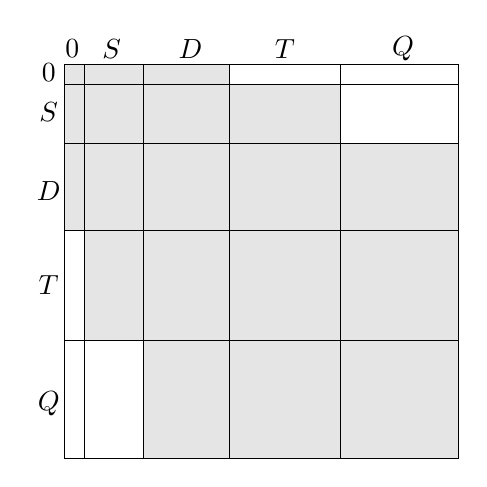
\begin{tikzpicture}[baseline={([yshift=-.5ex]current bounding box.center)},vertex/.style={anchor=base, minimum size=18pt, inner sep=2pt}]
 \draw (0,0.5) -- (0.5,0.5);
  \node[] at (0.1,5.2) {0};
  \node[] at (0.6,5.2) {$S$}; 
  \node[] at (1.6,5.2) {$D$};   
  \node[] at (2.8,5.2) {$T$}; 
  \node[] at (4.3,5.2) {$Q$};
  
  \filldraw[fill=white, draw=black] (0,0) rectangle (5,5);
  \filldraw[fill=black!10!white, draw=black] (0,5) rectangle (0.25,4.75);
  \filldraw[fill=black!10!white, draw=black] (0.25,5) rectangle (1.0,4.75);
    \filldraw[fill=black!10!white, draw=black] (1.0,5) rectangle (2.1,4.75);
	\filldraw[fill=white, draw=black] (2.1,5) rectangle (3.5,4.75);
	\filldraw[fill=white, draw=black] (3.5,5) rectangle (5,4.75);

  \filldraw[fill=black!10!white, draw=black] (0,4.75) rectangle (0.25,4.0);
  \filldraw[fill=black!10!white, draw=black] (0.25,4.75) rectangle (1.0,4.0);
    \filldraw[fill=black!10!white, draw=black] (1.0,4.75) rectangle (2.1,4.0);
	\filldraw[fill=black!10!white, draw=black] (2.1,4.75) rectangle (3.5,4.0);
	\filldraw[fill=white, draw=black] (3.5,4.75) rectangle (5,4.0);

  \filldraw[fill=black!10!white, draw=black] (0,4.0) rectangle (0.25,2.9);
  \filldraw[fill=black!10!white, draw=black] (0.25,4.0) rectangle (1.0,2.9);
    \filldraw[fill=black!10!white, draw=black] (1.0,4.0) rectangle (2.1,2.9);
	\filldraw[fill=black!10!white, draw=black] (2.1,4.0) rectangle (3.5,2.9);
	\filldraw[fill=black!10!white, draw=black] (3.5,4.0) rectangle (5,2.9);

  \filldraw[fill=white, draw=black] (0,2.9) rectangle (0.25,1.5);
  \filldraw[fill=black!10!white, draw=black] (0.25,2.9) rectangle (1.0,1.5);
    \filldraw[fill=black!10!white, draw=black] (1.0,2.9) rectangle (2.1,1.5);
	\filldraw[fill=black!10!white, draw=black] (2.1,2.9) rectangle (3.5,1.5);
	\filldraw[fill=black!10!white, draw=black] (3.5,2.9) rectangle (5,1.5);

  \filldraw[fill=white, draw=black] (0,1.5) rectangle (0.25,0);
  \filldraw[fill=white, draw=black] (0.25,1.5) rectangle (1.0,0);
    \filldraw[fill=black!10!white, draw=black] (1.0,1.5) rectangle (2.1,0);
	\filldraw[fill=black!10!white, draw=black] (2.1,1.5) rectangle (3.5,0);
	\filldraw[fill=black!10!white, draw=black] (3.5,1.5) rectangle (5,0);

  \node[] at (-0.2,4.9) {0};
  \node[] at (-0.2,4.4) {$S$};
  \node[] at (-0.2,3.4) {$D$};
  \node[] at (-0.2,2.2) {$T$};  
  \node[] at (-0.2,0.7) {$Q$};    
  \end{tikzpicture}
\end{equation}
As you can see, only the diagonal blocks and determinant connected by two or less substitutions are nonzero.
This means that the FCI matrix is very sparse.
To be more precise, for each row of the matrix, there will be as many elements as the number of singly and doubly substituted determinants, which is of the order of (neglecting spin and spatial symmetry)
\begin{equation}
N (2K - N) + \frac{1}{4} N^2 (2K - N)^2.
\end{equation}
Since the number of rows contains of the order of $\binom{2K}{N}$ elements, we can see that the number of nonzero elements divided by the number of matrix elements is
\begin{equation}
\text{fraction of nonzero elements} = \frac{N (2K - N) + \frac{1}{4} N^2 (2K - N)^2}{\binom{2K}{N}}.
\end{equation}
This quantity becomes smaller as $N$ and $K$ increase showing that $\textbf{H}$ is mostly empty.

\section{Iterative solution of the FCI equations}

In practical applications of FCI, it is impossible to store the full Hamiltonian matrix.
Instead, one uses a \textbf{direct} diagonalization algorithm that requires storage of only several trial coefficient vectors.
To see how direct algorithms work, suppose that we have a good initial guess to the FCI vector, $\tilde{\mathbf{c}}$, and that the exact eigenvector can be written as
\begin{equation}
\mathbf{c} = \tilde{\mathbf{c}} + \delta \mathbf{c}.
\end{equation}
From this approximate eigenvector we can compute an approximate energy $\tilde{E}$
\begin{equation}
\tilde{E} = \frac{\tilde{\mathbf{c}}^T
 \mathbf{H}\tilde{\mathbf{c}}}{\tilde{\mathbf{c}}^T \tilde{\mathbf{c}}}
\end{equation}
and write $E = \tilde{E} + \delta E$, where $\delta E$ is the energy error with respect to the eigenvalue $E$.
Substitute these quantity in the Schr\"{o}dinger equation ($\mathbf{Hc} = E\mathbf{c}$) gives
\begin{equation}
\mathbf{H}(\tilde{\mathbf{c}} + \delta \mathbf{c}) = E (\tilde{\mathbf{c}} + \delta \mathbf{c}),
\end{equation}
from which we get
\begin{equation}
(\mathbf{H} - \tilde{E} - \delta E)\delta \mathbf{c} =-
(\mathbf{H} - \tilde{E} - \delta E) \tilde{\mathbf{c}}
= -(\mathbf{H} - \tilde{E}) \tilde{\mathbf{c}} + \delta E \tilde{\mathbf{c}}.
\end{equation}
Ignoring $\delta E$, we can write an equation for $\delta \mathbf{c}$ that reads as
\begin{equation}
\delta \mathbf{c} = -(\mathbf{H} - \tilde{E})^{-1}(\mathbf{H} - \tilde{E}) \tilde{\mathbf{c}}.
\end{equation}
The inverse $(\mathbf{H} - \tilde{E})^{-1}$ can be simplified by retaining only the diagonal part of $\mathbf{H}$ ($\mathbf{H}_\mathrm{d}$) to get
\begin{equation}
\delta \mathbf{c} = -(\mathbf{H}_\mathrm{d} - \tilde{E})^{-1}(\mathbf{H} - \tilde{E}) \tilde{\mathbf{c}}.
\end{equation}
This equation shows that if we want to improve the trial eigenvector, we just need to evaluate an expression in which only the product, $\mathbf{H}\tilde{\mathbf{c}}$, appears. This quantity is usually called the \textbf{sigma vector} and it is indicated with $\boldsymbol{\sigma} = \mathbf{H}\tilde{\mathbf{c}}$.
Approaches based on direct diagonalization methods have extended the domain of FCI from several thousand determinants to several billions.

\end{document}

